\documentclass{article}

\usepackage{amsmath, amsthm, amssymb, amsfonts}
\usepackage{thmtools}
\usepackage{graphicx}
\usepackage{setspace}
\usepackage{geometry}
\usepackage{float}
\usepackage{hyperref}
\usepackage[utf8]{inputenc}
\usepackage[english]{babel}
\usepackage{framed}
\usepackage[dvipsnames]{xcolor}
\usepackage{tcolorbox}

\colorlet{LightGray}{White!90!Periwinkle}
\colorlet{LightOrange}{Orange!15}
\colorlet{LightGreen}{Green!15}

\newcommand{\HRule}[1]{\rule{\linewidth}{#1}}

\declaretheoremstyle[name=Theorem,]{thmsty}
\declaretheorem[style=thmsty,numberwithin=section]{theorem}
\tcolorboxenvironment{theorem}{colback=LightGray}

\declaretheoremstyle[name=Proposition,]{prosty}
\declaretheorem[style=prosty,numberlike=theorem]{proposition}
\tcolorboxenvironment{proposition}{colback=LightOrange}

\declaretheoremstyle[name=Principle,]{prcpsty}
\declaretheorem[style=prcpsty,numberlike=theorem]{principle}
\tcolorboxenvironment{principle}{colback=LightGreen}

\theoremstyle{definition}
\newtheorem{definition}{Definition}[section]

\theoremstyle{remark}
\newtheorem*{remark}{Remark}

\newcommand{\argmin}{\mathop{\mathrm{argmin}}}
\newcommand{\argmax}{\mathop{\mathrm{argmax}}}
\newcommand{\minimize}{\mathop{\mathrm{minimize}}}
\newcommand{\maximize}{\mathop{\mathrm{maximize}}}
\newcommand{\st}{\mathop{\mathrm{subject\,\,to}}}
\newcommand{\tab}[1][1cm]{\hspace*{#1}}

\def\R{\mathbb{R}}
\def\E{\mathbb{E}}
\def\P{\mathbb{P}}
\def\S{\mathbb{S}}
\def\Cov{\mathrm{Cov}}
\def\Var{\mathrm{Var}}
\def\half{\frac{1}{2}}
\def\sign{\mathrm{sign}}
\def\supp{\mathrm{supp}}
\def\th{\mathrm{th}}
\def\tr{\mathrm{tr}}
\def\dim{\mathrm{dim}}
\def\dom{\mathrm{dom}}


\def\hwnum{3}


\setstretch{1.2}
\geometry{
    textheight=9in,
    textwidth=5.5in,
    top=1in,
    headheight=12pt,
    headsep=25pt,
    footskip=30pt
}

% ------------------------------------------------------------------------------

\begin{document}

% ------------------------------------------------------------------------------
% Cover Page and ToC
% ------------------------------------------------------------------------------

\title{ \normalsize \textsc{}
		\\ [2.0cm]
		\HRule{1.5pt} \\
		\LARGE \textbf{\uppercase{3D Deep Learning Approaches}
		%\HRule{2.0pt} \\ [0.6cm] \LARGE{Subtitle}
        \vspace*{10\baselineskip}}
		}
\date{}
\author{\textbf{Author} \\ 
		Vinitra Muralikrishnan \\
		11th March, 2024}

\maketitle
\newpage

\tableofcontents
\newpage

% ------------------------------------------------------------------------------

\section{Multi View Approach}

\begin{itemize}
    \item Image based networks can process individual shape renderings
    \item They are basically convolution layer networks combined for reasoning across multiple rendered shape views.\\
    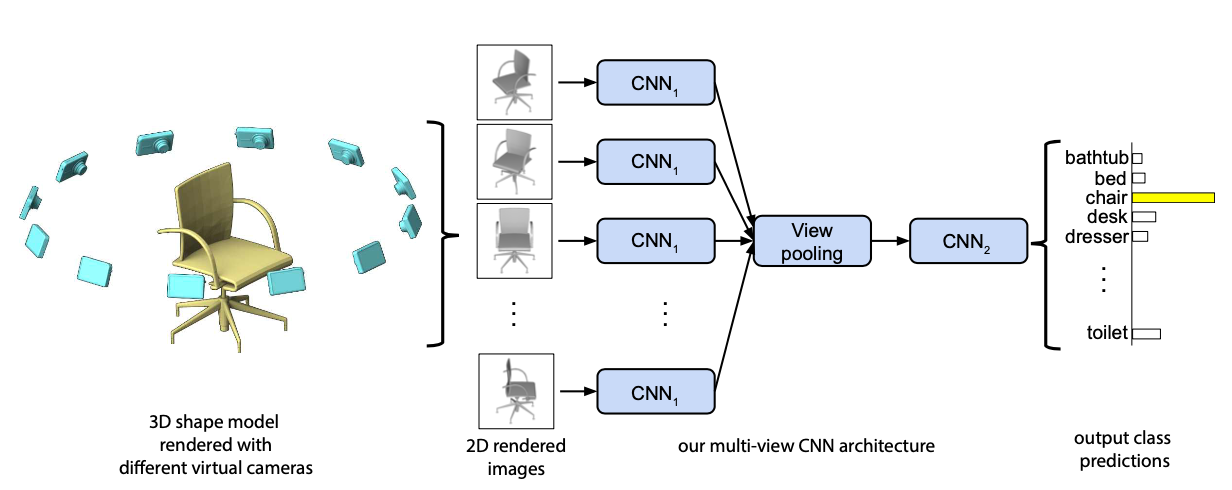
\includegraphics[width=5in]{img/mvn.png}
    \item For classification
    \begin{itemize}
        \item Get renderings of a shape from different viewpoints. Cover different camera rotations, distances, viewpoints
        \item Feed all views of a shape to an FCN.
        \item For every view get the predicted probability of all labels
        \item Aggregate the probability across all views. The aggregator can be max or mean pooling
        \item The maximum value across all labels then would be the prediction
    \end{itemize}
    \item For segmentation
    \begin{itemize}
        \item For each input shape, infer a set of viewpoints that covers the maximum (99.99999\%) surface
        \item Cover each view across multiple distances and with different camera rotations (to cover different orientations as CNN is not rotation invariant)
        \item Render shape images (normal dot view vector) encoding surface normals
        \item Render depth images encoding surface position relative to the camera
        \item Feed each pair of images to an FCN (fully convoluted networks)
        \item The views are not ordered so FCNs can share parameters
        \item For each input, the FCN will output the confidance map per part label
        \item The confidence maps then can be aggregated and projected to get a single surface map
        \item For each surface element, final all pixels painted by it in all views. Surface confidence is max of these pixel confidences per label
    \end{itemize}
    \item For correspondences
    \begin{itemize}
        \item For every shape, patches of the shape are generated and such patches are fed into an FCN
        \item The FCN gives shape descriptors for each of the "patches"
        \item View pooling and dimensionality reduction is done to prune no of datapoints or features identified between the 2 shapes
        \item Contrastive loss is applied on both shape descriptors and points of difference are identified
        \item Example: \href{https://www.cs.cmu.edu/~rsalakhu/papers/oneshot1.pdf}{Siamese Architecture}
    \end{itemize}
    \item Pros
    \begin{itemize}
        \item Excellent performance for shape classification
        \item Re use of powerful 2D image architectures
        \item Use of pretrained models
        \item Good resolution for shape analysis
    \end{itemize}
    \item Cons
        \begin{itemize}
            \item Cannot process invisible areas 
            \item Can be slow 
            \item 2d proximity is different from 3d proximity after projection
            \item Heuristics for viewpoint positions/orientations need to be carefully designed. Optimal heuristics need to be identified every time
        \end{itemize}
\end{itemize}

%\begin{definition}
    %This is a definition
%\end{definition}

%\begin{theorem}
    %This is a theorem.
%\end{theorem}

%\begin{proposition}
    %This is a proposition.
%\end{proposition}

%\begin{principle}
    %This is a principle.
%\end{principle}

%% Maybe I need to add one more part: Examples.
%% Set style and colour later.

%\subsection{Pictures}

%\begin{figure}[htbp]
    %\center
    %%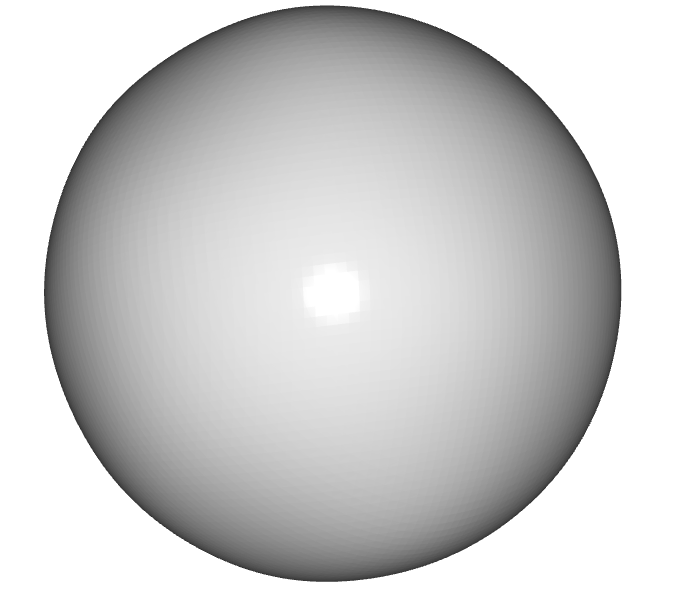
\includegraphics[scale=0.06]{img/photo.png}
    %\caption{Sydney, NSW}
%\end{figure}

%\subsection{Citation}

%This is a citation\cite{Eg}.

%\newpage

% ------------------------------------------------------------------------------
% Reference and Cited Works
% ------------------------------------------------------------------------------

\bibliographystyle{IEEEtran}
\bibliography{References.bib}

% ------------------------------------------------------------------------------

\end{document}
